% ==================================================================
% Graham Pellegrini — CV in LaTeX (single column)
% Save as main.tex. Compile with xelatex (recommended) or pdflatex.
% ==================================================================
\documentclass[11pt,a4paper]{article}

% ---------- Encoding & Fonts ----------
\usepackage[utf8]{inputenc}
\usepackage[T1]{fontenc}
\usepackage{lmodern}
\usepackage{microtype}

% ---------- Graphics & Color ----------
\usepackage{graphicx}
\usepackage[dvipsnames]{xcolor}
\usepackage{tikz}
\usepackage{fontawesome5}

% ---------- Layout ----------
\usepackage[a4paper,top=0cm,left=1.6cm,right=1.6cm,bottom=1.6cm,includefoot]{geometry}

\usepackage{enumitem}
\setlist[itemize]{leftmargin=1.2em,itemsep=0.2em,topsep=0.2em}
\usepackage{tabularx}
\usepackage{array}
\usepackage{titlesec}
\usepackage[hidelinks]{hyperref}

% ---------- Styling helpers ----------
\definecolor{accent}{HTML}{2E86AB}   % Main blue for section headers
\definecolor{subaccent}{HTML}{5CB3D6}  % Lighter blue for subsection headers
\definecolor{text}{HTML}{222222}
\definecolor{muted}{HTML}{666666}
\definecolor{bannerbg}{HTML}{5CB3D6}  % Light blue for header
\definecolor{bannertext}{HTML}{FFFFFF}

\newcommand{\name}[1]{\textbf{\Large #1}}
\newcommand{\tagline}[1]{\textit{#1}}

% Section header style with underline
\titleformat{\section}{\large\bfseries\color{accent}}{ }{0pt}{}[\vspace{0.1em}\color{accent!40}\rule{\linewidth}{0.8pt}\vspace{0.4em}]

% Entry helper for dated items - with subsection styling
\newcommand{\entry}[3]{% org, dates, description
  \noindent\textbf{#1}\\[-1pt]
  \textcolor{muted}{#2}\\
  \color{text}#3\par\vspace{0.6em}}

% Photo command - using actual profile picture
\newcommand{\profilephoto}{%
  \begin{tikzpicture}
    \clip (0,0) circle (1.5cm);
    \node at (0,0) {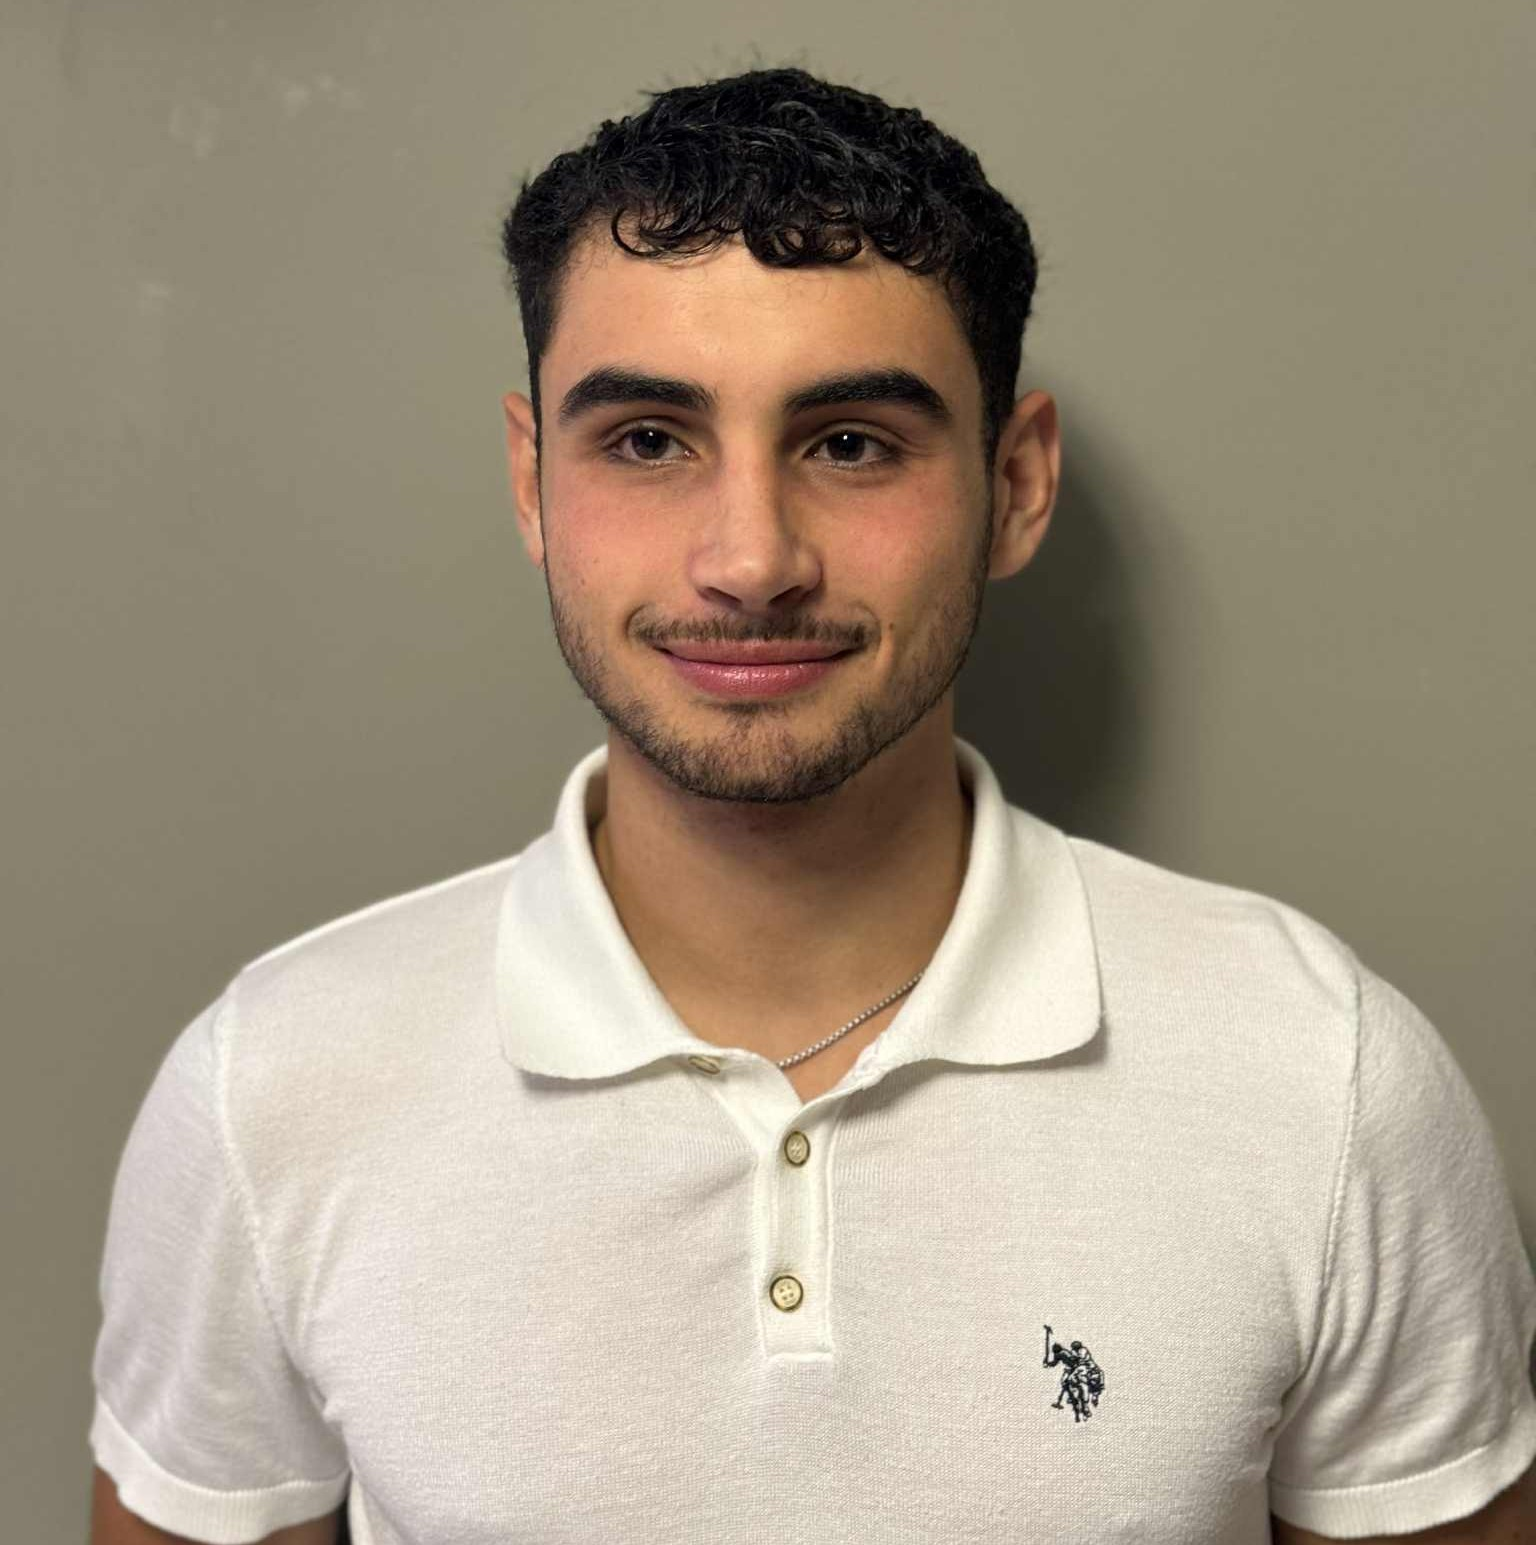
\includegraphics[width=3cm,height=3cm,keepaspectratio]{profile_picture.jpeg}};
  \end{tikzpicture}%
}

\begin{document}
\pagestyle{empty}
\color{text}
\setlength{\emergencystretch}{2em} % helps justification

% ===== Top banner with name, contact info and picture =====
% Using tikz to create full-width header with integrated photo
\begin{tikzpicture}[remember picture,overlay]
  % Blue background banner (increased height for contact info)
  \fill[bannerbg] (current page.north west) rectangle ([yshift=-4.5cm]current page.north east);
  
  % Profile picture (clipped to circle) positioned on the left side of the banner
  \begin{scope}
    \clip ([xshift=3cm,yshift=-2.25cm]current page.north west) circle (1.6cm);
    \node at ([xshift=3cm,yshift=-2.25cm]current page.north west) 
      {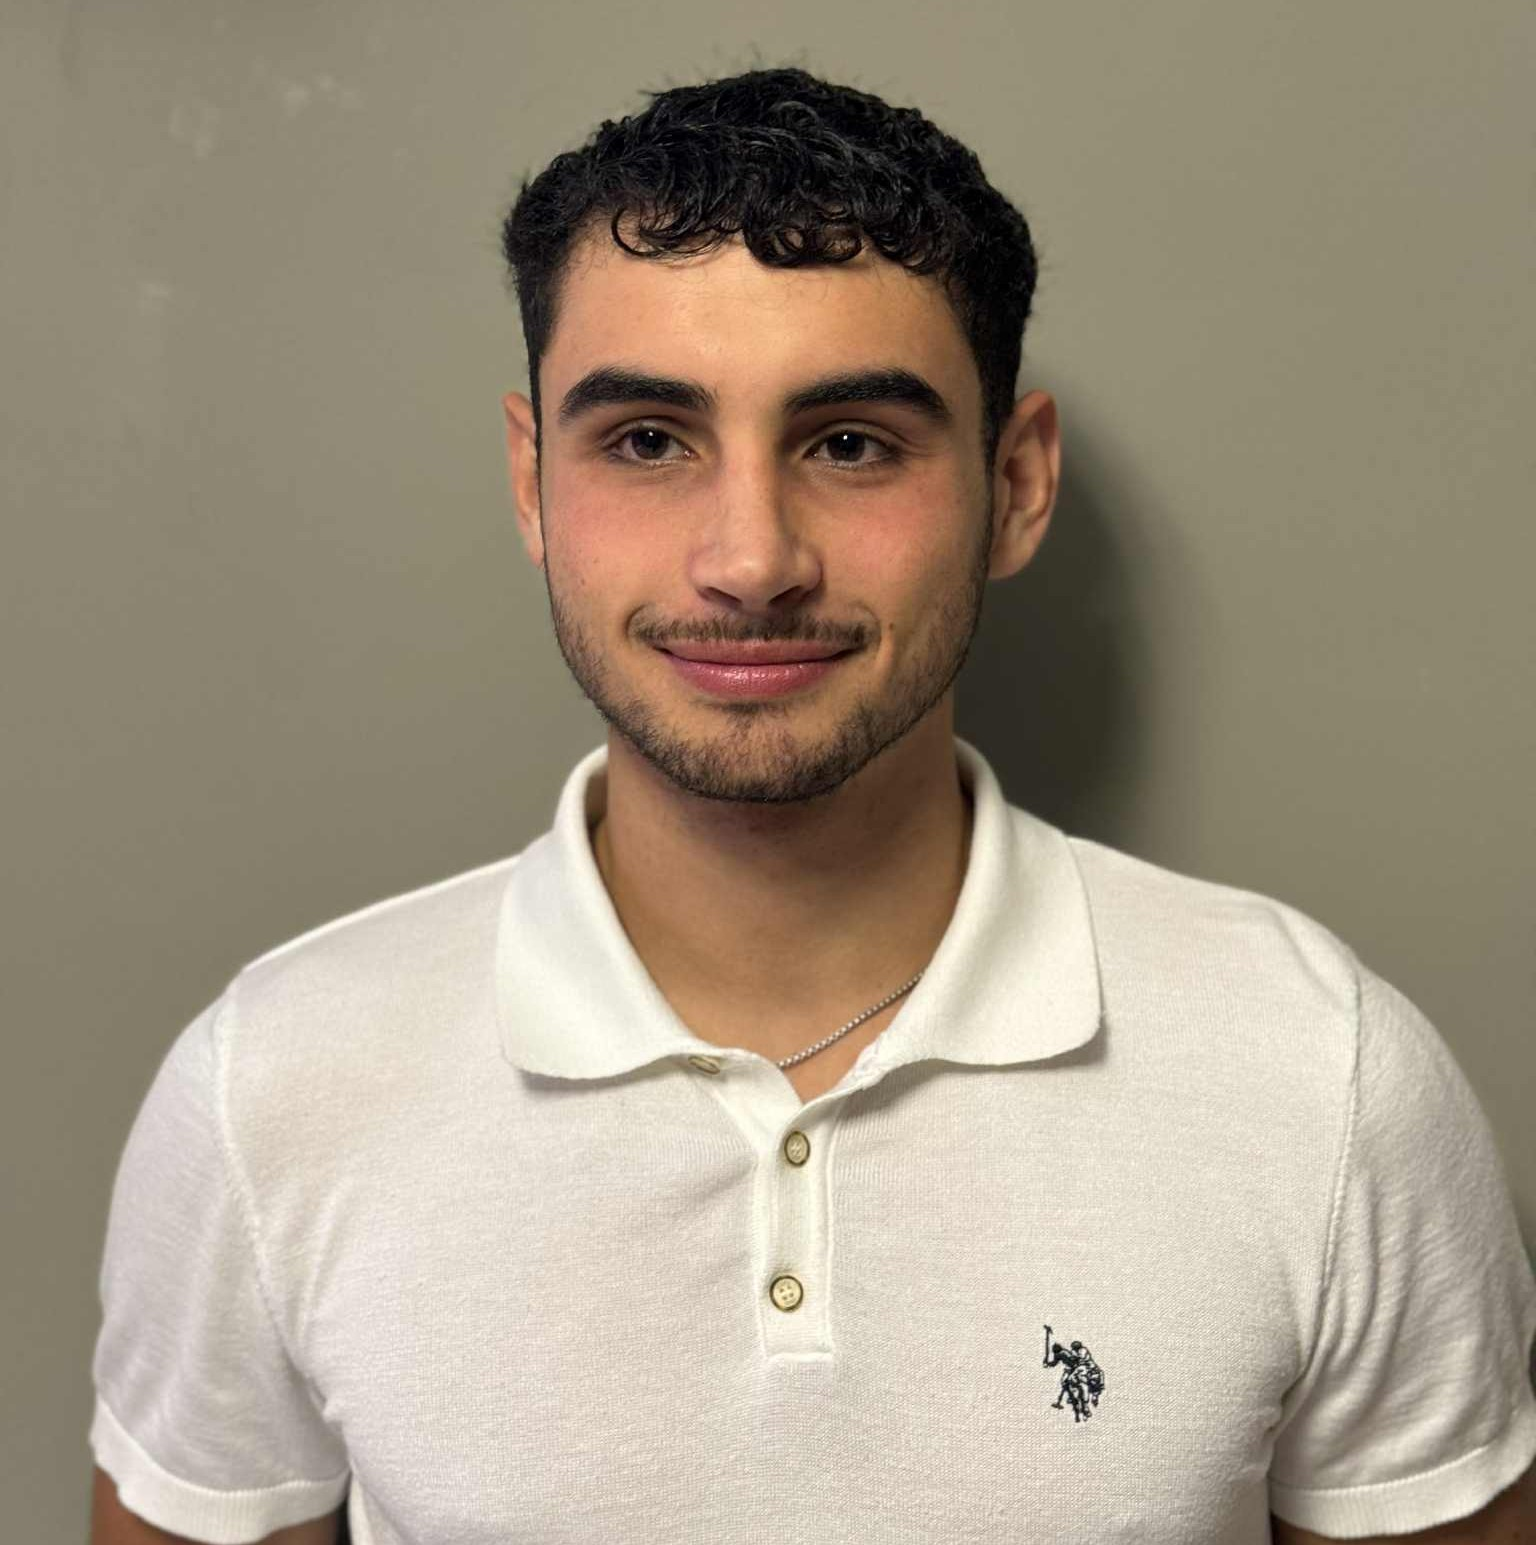
\includegraphics[width=3.2cm,height=3.2cm,keepaspectratio]{profile_picture.jpeg}};
  \end{scope}
  
  % White border around the photo
  \draw[bannertext,line width=2pt] ([xshift=3cm,yshift=-2.25cm]current page.north west) circle (1.6cm);
  
  % Name text positioned to the right of the photo
  \node[anchor=west,text=bannertext] at ([xshift=5.5cm,yshift=-1.5cm]current page.north west) 
    {\Huge\bfseries Graham Pellegrini};
  
  % Contact information below the name
  \node[anchor=west,text=bannertext] at ([xshift=5.5cm,yshift=-2.8cm]current page.north west) 
    {\large\href{mailto:grahammalta@gmail.com}{\faEnvelope} \hspace{0.8em}
     \href{tel:+35699760266}{\faPhone} \hspace{0.8em}
     \href{https://www.linkedin.com/in/graham-pellegrini-858690244/}{\faLinkedin} \hspace{0.8em}
     \href{https://github.com/GrahamPellegrini}{\faGithub}};
  
  % Address below contact icons
  \node[anchor=west,text=bannertext] at ([xshift=5.5cm,yshift=-3.5cm]current page.north west) 
    {\faMapMarker* \hspace{0.3em} {\small 9, Hibiscus, Triq Andre' Maurois, St Julians, STJ 1573, Malta}};
\end{tikzpicture}

\vspace*{4.5cm}
\color{text}

% ===== Single column content =====
\color{text}

\section*{Profile}
\textbf{DOB:} 23/10/2004\\
\textbf{Nationality:} Maltese\\

\noindent
Hardworking university student seeking internship opportunities to gain practical experience and broaden my skill set. I am a critical thinker who prioritises logic and a clear understanding of the problem at hand. Outside work and study, I am a national athlete representing Malta in the 200m \& 400m, who also enjoys scuba diving.

\section*{Work Experience}
\entry{Summer Intern, EY (Ernst \& Young)}{Summer 2023, 2024 \& 2025}{Three consecutive summer internships gaining experience with Microsoft cloud tools (Power Platform), learning the technology consulting role and how to work in a team working environment.}

\entry{Coach, MSC Summer Camp}{Aug 2024}{Coached young athletes, developing leadership and communication skills whilst sharing enthusiasm for sports.}

\section*{Education}
\entry{M.Sc. Artificial Intelligence, University of Malta, Msida}{Present}{Awaiting confirmation}

\entry{B.Sc. (Hons) Computer Engineering, University of Malta, Msida}{Oct 2022 — Jun 2025}{Second Upper Class Graduate\\ Final Year Project: Machine Learning Noise Cancellation
System (A)}
\pagebreak
\vspace*{2em}

\entry{MATSEC A-Level, Saint Aloysius College, Birkirkara}{Oct 2020 — May 2022}{\textbf{Advanced:}
\begin{itemize}
  \item Physics (B)
  \item Pure Mathematics (B)
\end{itemize}
\textbf{Intermediate:}
\begin{itemize}
  \item Computing (B)
  \item Accounting (B)
  \item English Language (C)
  \item Systems of Knowledge (A)
\end{itemize}}

\entry{MATSEC O-Level, St Michael's Foundation, San Gwann}{Oct 2007 — Jun 2020}{All Level 3: \begin{itemize}
  \item Maltese
  \item Religious Knowledge
  \item English Language
  \item English Literature
  \item Mathematics
  \item Physics 
  \item Accounting
  \item Computer Studies
  \item Economics
  \item German
\end{itemize}}

\section*{Other Certificates}
\begin{itemize}
  \item Certificate of Participation, 10th Malta Mathematics Olympiad (Apr 2019)
  \item ECDL (Jun 2020)
  \item Social Responsibility Programme (Salesians Senglea) completion (Jun 2022)
  \item Advanced and Open Water Diver (Aug 2022)
  \item Participation at the Basic Track on Quantum Computing, Qalypso Summer School (Sep 2022)
\end{itemize}
\pagebreak
\vspace*{2em}

\section*{\href{https://www.worldathletics.org/athletes/malta/graham-pellegrini-147123}{Athletics Profile}}

\textbf{Discipline:} Middle-distance sprints (200m \& 400m)\\
\textbf{Club:} Pembroke Athleta\\
\textbf{Coach:} Steve Camilleri\\

\noindent
\textbf{National Records:}
\begin{itemize}
  \item U18/U20 300m NR Holder (February 2023) - 34.42s
  \item U20/U23 200m NR Holder (April 2023) - 21.18s
  \item Open/U23/U20 400m NR  (June 2023 (broken 2025)) - 46.83s
  \item Open/U23 300m NR Holder (February 2024) - 33.15s
  \item Open/U23 400m Indoor NR Holder (February 2024) - 47.55s

\end{itemize}


\noindent \\
\textbf{Achievements \& Awards:}
\begin{itemize}
  \item ISF World School Championships Athletics, Croatia (May 2019)
  \item U18 Athlete of the Year (2020) \& (2021)
  \item Two Gold and One Silver Medalist GSSE (2022)
  \item University of Malta GSSE Commemoration
  \item Atlas Athlete of the Month (June 2023)
  \item Atlas Athlete of the Month (February 2024)
  \item Certificate of Achievement Mediterranean Games (May 2024)
  \item 77th Balkan Athletics Championship participation (May 2024)
\end{itemize}

\end{document}
